% !TEX root = ../Thesis.tex
\chapter{Background}

In this chapter we introduce the environment for which the word-gesture keyboard is mainly developed, some things about conventional and word-gesture keyboards in general and $\text{SHARK}^2$.

\section{vitrivr-VR and UnityVR}
vitrivr\footnote{https://vitrivr.org/} is an ``open source full stack content-based multimedia retrieval system''\footnote{https://dbis.dmi.unibas.ch/research/projects/vitrivr-project/}. It supports video, image, audio and 3D collections. It also features a very broad set of query paradigms that are supported. vitrivr is developed by the Database and Information Systems group\footnote{https://dbis.dmi.unibas.ch} (dbis) of the university of Basel. For our thesis, we use the VR part of vitrivr, namely vitrivr-VR, which is being developed in Unity\footnote{https://unity.com}.

Unity is a tool for developers where one can create projects in 2D, 3D and VR. To a certain degree Unity is free to use. Developers can provide assets and Unity packages. These can be either free to use or have to be bought. Another developer then can import and use these in their own Unity projects. The main language used in Unity is C\#. A developer can write such C\# scripts and if needed attach them to objects in a scene. These scripts can control the objects and what they are doing when a user interacts with them or something particular happens. 

\section{Conventional Keyboard}
In this thesis, when we talk about a conventional keyboard, we do not look at its type of construction, at any special layouts or whether it is a mechanical keyboard or not. We define the term ``conventional keyboard'' as the most used keyboard type, the one where a user has to input every single letter by pressing or tapping a single key. There are two different kinds of conventional keyboards. One is the physical variant. This one is used for most desktop and laptop computers. The other variant is a so-called soft keyboard. This is an on-screen conventional keyboard that is mostly used with phones, tablets and other touchscreen-based devices. It has the same functionality as the physical conventional keyboard but instead of pressing a physical key, one has to tap on the screen at the right place.
%On desktop and laptop computers we normally use such a conventional keyboard. One thing that might be different in some countries is the layout. But that does not change the functionality. Conventional keyboards are also the most used keyboard for phones, tablets and other touchscreen-based devices. The only difference is that we do not press physical keys, but tap on the screen, where a certain key is. These keyboards work really well for text input with the previously mentioned devices. 

\subsection{Disadvantages in VR/AR}
When it comes to VR and AR, it seems that this is not the best method to input text. One reason for this is that tactile feedback and accurate finger tracking is currently lacking in VR and AR. While this could be improved during the next years, it is not really there yet. Another reason is the size of such keyboards in VR. A user has to tap on the keys with their controllers. If the keys are too close together, it might cause a problem in recognizing which one the user wants to press. Therefore, there needs to be either bigger keys or bigger spaces between two adjacent keys. This results in a bigger keyboard, which in turn ends in more needed movement with the arms. If the user has to move their arms a lot to input some text, this can quickly become exhausting.

\section{Word-Gesture Keyboard}
A word-gesture keyboard may look pretty much the same as a conventional keyboard but works quite different. First of all, it does not exist in a hardware version like the conventional keyboard does. It is more like the soft keyboard version on a screen. Independent of the details of the implementation, every word-gesture keyboard works with gestures. This means, instead of tapping on single keys, the user has to draw one line or a shape on the keyboard. This will then be evaluated by an algorithm. It determines the closest word, the one with the most similar shape seen from different aspects, from a lexicon. For example, to input the word ``science'', the user has to put the finger on the screen, where the ``s-key'' is displayed. Then they have to move, with the finger still on the screen, to the respective adjacent key with the correct character. At the end, the user has to take away their finger from the screen at the ``e-key''. If the gesture is more or less good, the algorithm behind should now be able to calculate that ``science'' is the word the user intended to write. But if the gesture is done bad, it can happen that a wrong word is being calculated. 

\subsection{$\text{SHARK}^2$}
\label{SHARK2}
$\text{SHARK}^2$ is a ``large vocabulary shorthand writing system for pen-based computers'' \cite{Kristensson2004SHARK2AL} developed by Shumin Zhai and Per-Ola Kristensson. It can compare a user inputted graph with a perfect graph of any word in a given lexicon.
\begin{figure}[H]
    \centering
    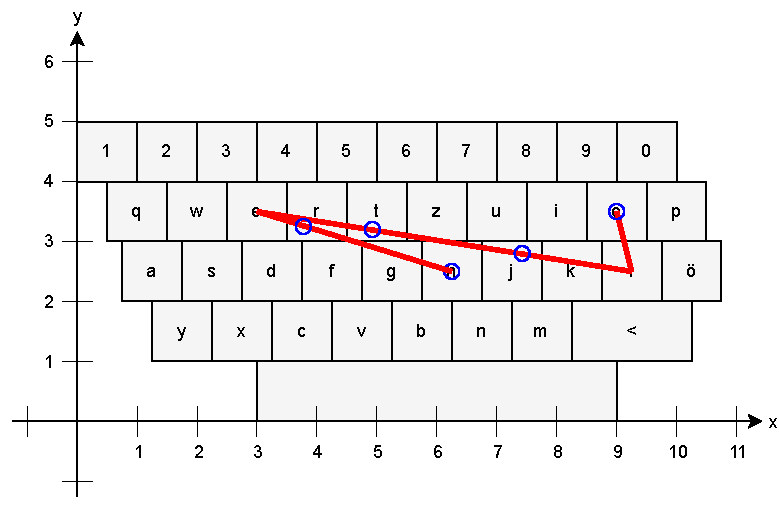
\includegraphics[width=0.75\textwidth]{BAPerfectGraph.pdf}
    \caption{Perfect graph of the word "hello" with red lines. The 5 blue points show the sample points, if the graph was sampled with a number $N = 5$.}
    \label{fig:PerfectGraph}
\end{figure}
A perfect graph for a word is the graph that is produced if we start from the center of the word's first letter on the keyboard. Then we draw a straight line to the center of the next letter of the word and so on, until we reach the last letter. The resulting perfect graph for the word ``hello'' can be seen in \Cref{fig:PerfectGraph}. A user inputted graph is the graph the user draws with their gesture on the keyboard. $\text{SHARK}^2$ then can find the word with the most similar perfect graph compared to the user input. To achieve this, it uses a multi-channel recognition system. The most important part are two core channels, a shape recognizer and a location recognizer, where different aspects of the graphs get looked at. There is also a channel that brings language information into the calculation. Additionally, the system uses some other tricks to achieve the best possible results.

\subsubsection{Preconditions}
The $\text{SHARK}^2$ system needs a lexicon that should be in the order of 10'000 words. Such a lexicon can be obtained through different methods. For example, the lexicon used to test $\text{SHARK}^2$ was mined from one of the authors' emails, but it could also just be a standard dictionary. For all the words in the lexicon, their perfect graphs have to be stored as well. Zhai and Kristensson \cite{Kristensson2004SHARK2AL} do not mention how they store these, but it would make sense, to only store $N$ points for each graph, with $N$ being the number of points that samples one. This can be justified by the fact that for later calculations with the graphs only these $N$ points are needed per graph and not more.

\subsubsection{Template Pruning}
First of all, $\text{SHARK}^2$ uses template pruning. It compares the start and end positions of the perfect graph of each word in the lexicon with the input gesture from the user, both being normalized in shape and location. If either the start-to-start or end-to-end distance is bigger than a given threshold, the checked word will be discarded and not further considered.

\subsubsection{Shape Channel Recognition}
\label{normalize}
The next step is to apply the shape recognizer. It compares the shapes of the perfect graph of each word in the lexicon with the user inputted graph. For this, an amount of $N$ sampling points has to be calculated for every graph. These $N$ points need to be equidistant. An example of this sampling can be seen in \Cref{fig:PerfectGraph}.
\begin{figure}[H]
    \centering
    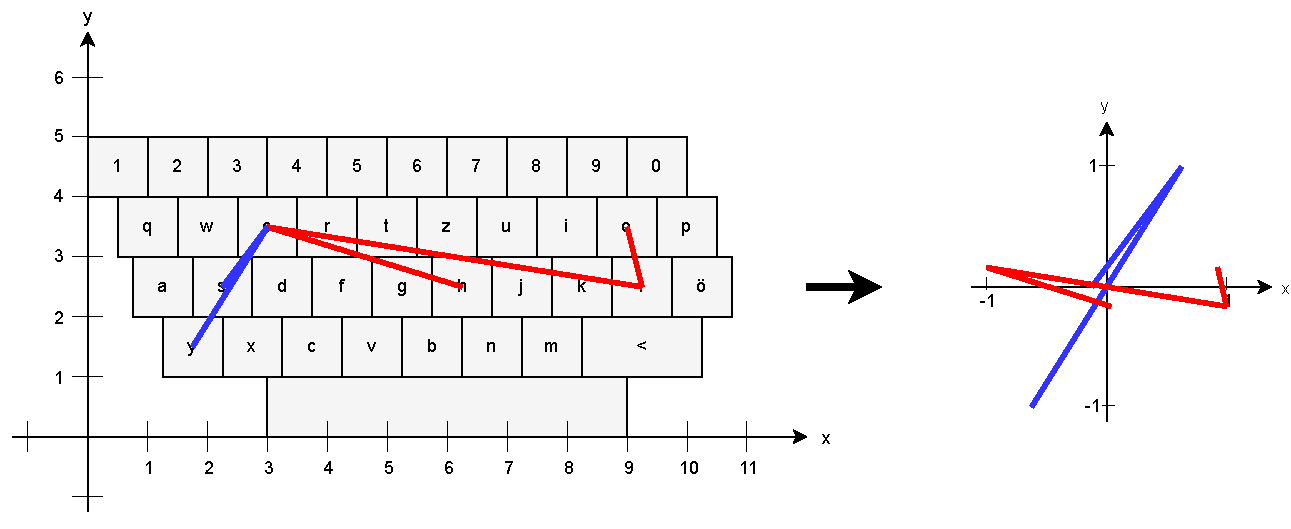
\includegraphics[width=0.75\textwidth]{BAFigNorm.pdf}
    \caption{Normalization of the perfect graphs of the words ``yes'' and ``hello'' to a predetermined length of 2}
    \label{fig:Norm}
\end{figure}
Then they have to be normalized in scale and location as it is done in \Cref{fig:Norm}. First of all, the middle point $m$ of every graph's bounding box has to be calculated. Further, $m$ has to be subtracted from every point, because this sets the middle point of the bounding box to $(0,0)$, thus normalizes it in location. Then the graphs are all normalized in scale by scaling the largest side of the graph's bounding box to a predetermined length $L$: 
\begin{equation}
    s = \frac{L}{\text{max}(W,H)}
\end{equation}
$W$ and $H$ are the width and height of the graph's bounding box.  Then, all points' positions have to be multiplied by $s$ to get the normalized positions. 
\begin{figure}[H]
    \centering
    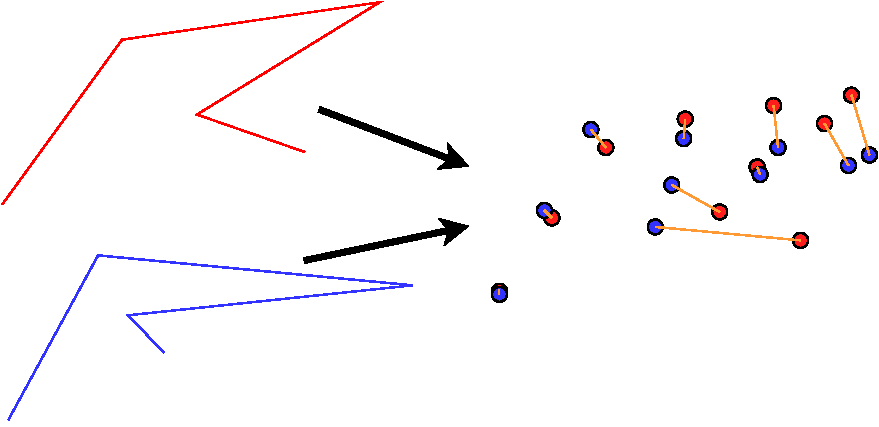
\includegraphics[width=0.75\textwidth]{BAFigDist.pdf}
    \caption{Calculating the distance of two random graphs. This is the summed up distance of all distances between the pairs of points. A pair consists of two i-th points, one from every graph, where $i \in \{1,N\}$. }
    \label{fig:Distance}
\end{figure}
Now, the distance between the normalized user inputted graph and every word's normalized perfect graph has to be calculated. To do so, we use the following formula:
\begin{equation}
    x_S = \frac{1}{N}\sum_{i = 1}^{N}\left\lVert u_i - t_i\right\rVert_2
\end{equation}
where $u_i$ is the i-th point of the user inputted graph and $t_i$ the i-th point of a word's perfect graph. The result $x_S$ is the so-called ``proportional shape matching distance'' \cite{Kristensson2004SHARK2AL}.\\

Now, one could think that this is enough and with the application of the template pruning and shape channel recognition the word is perfectly determined. This is not the case. The authors state that words can have a similar or even the same shape as other words. They call these word pairs ``confusion pairs''. They found that, for example, on an ATOMIK layout with a lexicon of 20'000 words, 1'117 confusion pairs occur, if the starting and ending positions are not considered. If these are also considered with the shape, there is still a total of 537 confusion pairs. 
%Each channel alone from the system developed by Zhai and Kristensson \cite{Kristensson2004SHARK2AL} does not necessarily have enough power, but all the channels together can detect the right word.

\subsubsection{Location Channel Recognition}
To avoid a lot of these confusion pairs, the authors are using a second channel, the location recognizer. For the following formulas and calculations, the normalization of the graphs is not needed anymore. As the name states, it is about the location, where the graph lies in a coordinate system.\\
They use an algorithm that computes the distance of the user inputted graph $u$ to the perfect graph $t$ of every word in the lexicon. The location channel distance is defined as:
\begin{equation}
    x_L = \sum_{i = 1}^{N}\alpha(i)\delta(i)
    \label{eqn:locationformula}
\end{equation}
where $N$ is the number of points used to sample a graph and $\alpha(i)$ with $i \in (1,N)$ are weights for the different point-to-point distances, such that $\sum_{i = 1}^{N}\alpha(i) = 1$. These weights can be set in various ways. For $\text{SHARK}^2$ the authors use a function that gives the lowest weight to the middle point-to-point distance. The weight increases linearly towards the two ends for the other point-to-point distances. Another way could be through training with a large amount of data. Lastly, $\delta(i)$ is defined by the following formula:
\begin{equation}
    \delta(i) =
        \begin{cases}
            0, & D(u,t) = 0 \land D(t,u) = 0 \\
            \left\lVert u_i - t_i \right\rVert_2, & \text{otherwise}
        \end{cases}
\end{equation}
where $u_i$ is the i-th point of $u$ and $t_i$ the i-th point of $t$. Further, $D$ is defined as:
\begin{equation}
    D(p,q) = \sum_{i = 1}^{N}\text{max}(d(p_i,q) - r,0)
\end{equation}
where $r$ is the radius of a key on the keyboard and $d$ is defined as:
\begin{equation}
    d(p_i,q) = \text{min}(\left\lVert p_i - q_1 \right\rVert_2, \left\lVert p_i - q_2 \right\rVert_2, \dots, \left\lVert p_i - q_N\right\rVert_2)
\end{equation}

For all these formulas $N$ is the number of points used to sample a graph. The ``trick'', for which the authors use these formulas, is quite simple. They state that they form something like an ``invisible'' tunnel of one key width that contains all keys used to write a certain word. A perfect distance score of zero is given, when all the sampled points of the user inputted graph lie within the tunnel of $t$. If this is not the case, the distance score for $t$ with respect to the user inputted graph $u$ is set to the sum of the spatial point-to-point distances. This means $N$ distances have to be calculated and summed up. These are the distances between the i-th point of $u$ and the i-th point of $t$ for $i \in \{1,N\}$, as seen in the example in \Cref{fig:Distance}.

\subsubsection{Channel Integration}
With the two distances $x_S$ and $x_L$, the most probable word, the user intended to write, can be calculated pretty well. The authors assume that the distance from a user inputted graph to the perfect graph of a word follows a Gaussian distribution. This means, if the user inputted gesture has distance $x$ to a perfect graph of a word $w$, the probability that $w$ is the intended word can be calculated using the Gaussian probability density function:
\begin{equation}
    p(x) = \frac{1}{\sigma\sqrt{2\pi}}\exp\left[{-\frac{1}{2}}\left(\frac{x-\mu}{\sigma}\right)^2\right]
    \label{eqn:gaussian}
\end{equation}
One important thing here is that this calculation has to be performed two times per word because it has to be done for $x_S$ and $x_L$. They set $\mu = 0$ and $\sigma$ can be obtained through training from large amount of data. Here, $\sigma$ can be seen as the sensitivity of a channel. If, for example, $\sigma$ is equal to one key radius, the words, whose perfect graphs have a greater distance to the user inputted graph than one key width, have practically zero probability of being the intended word. For $\text{SHARK}^2$ the authors use $\sigma$ as parameter to adjust the weight of contribution of each channel. They also use $\sigma$ for further pruning. They discard all candidate words, whose distance $x$ is bigger than 2$\sigma$. For the candidate words $w \in W$, that have not been discarded until now, the marginalized probability to be the intended word is: 
\begin{equation}
    p'(w) = \frac{p(x)}{\sum\limits_{i \in W}p(i)}
\end{equation}
%where p(i) is used from formula above ((p(x))
Note that this calculation also needs to be performed twice per word, once for the location channel and once for the shape channel. The last step of the channel integration is to integrate the probabilities from the two channels using Bayes' rule:
\begin{equation}
    c(w) = \frac{p'_S(w)p'_L(w)}{\sum\limits_{i \in W_S \cap W_L}p'_S(i)p'_L(i)}
\end{equation}
The final result $c(w)$ is now the confidence score for the word $w$.

\subsubsection{Further Steps To Improve The Results}
There are also some further steps that can be made but we do not implement in our algorithm. In this section, we discuss briefly about these.
\paragraph{Dynamic Channel Weighting by Gesturing Speed}\
\label{gesturing speed}\\
The authors say that the user can draw a graph either on visual guidance from the keyboard (looking for the next letter of a word on the keyboard) or recall from memory. A graph drawn by visual guidance results in a higher location distance score than a graph drawn from memory recall. If a user draws a graph by memory recall, the location distance score will be poor and the focus lays more on the shape. Therefore, they suggest a dynamic weighting of the two channels. In general, graphs drawn by memory recall are faster than visual guided ones. Hence, the gesture completion time should tell how heavy each of the two channels should be weighted in the final selection. The time to complete a graph for a word obviously depends on its length and complexity. The authors use Fitts' law to calculate the normative writing time for a perfect graph. This law predicts that the time one needs to move to a target area is a function of the ratio between the distance to the target and the width of the target. They use this result together with the actual graph production time to modify $\sigma$ used in formula \ref{eqn:gaussian}.
\paragraph{Using Language Information}\ \\
The authors achieved quite good performance with the two core channels, but there still might be conflicting words. To prevent these, the authors suggest to also use language context. For $\text{SHARK}^2$ smoothed bigrams are used as the language model, which is then used to rearrange the N-best list of words received before (the N words with the highest confidence score).

\subsubsection{Other VR Input Methods}
Later on, we will need the text input methods used by Boletsis and Kongsvik \cite{Boletsis2019ControllerbasedTT}. Therefore, we briefly introduce them here.\\

Raycasting keyboard: One of the most popular VR input method. A user casts a ray from their controller and has to aim for the keyboard. When aiming at a key, a button of the controller can be pressed to input a character. In this case, it is a two-handed one, which means a user can use both hands simultaneously.\\

Drum-like keyboard: The controllers are drumsticks. A user has to click on the keyboard keys with these sticks as they were their hands.\\

Head-directed input keybpard: The user controls a pointer with their head movement. They have to aim for a key and then press a certain button on the controller to select it.\\

Split keyboard: A virtual keyboard is split in two parts, where each is assigned to a controller. The keyboard keys can be selected by the touch-sensitive trackpad of the controllers (Vive controllers) and characters can be inputted by pressing the trackpad button.\\

All of these keyboards have in common that only single characters can be inputted and not whole words as one.
\label{sec:other_keyboards}